\section{Tafeldetektierung}

Das folgende Kapitel befasst sich mit dem ersten Schritt in der automatisierten Analyse der Grabungsfotos: der Erkennung der Schiefertafeln.\\
Zunächst sollen die Tafeln vorgestellt und die Probleme bei der Detektion erörtert werden. Im Anschluss werden verschiedene Möglichkeiten der Erkennung präsentiert. Schließlich werden mehrere angewandte Methoden erörtert und die erzielten Ergebnisse vorgestellt.

\subsection{Die Tafeln und ihre Tücken}

\subsubsection{Die Tafeln}

Die Verwendung von Tafeln zur Dokumentation von Fund- und Grabungsarealen ist in allen, im weitesten Sinne grabenden, Wissenschaften weit verbreitet (Vgl. Bildquellen) . So setzt auch die Archäologie diese Methode ein. Dabei werden neben den zu dokumentierenden Gebieten verschiedenste Formen von Tafeln oder Schildern platziert, auf denen Zeit und Ort der Aufnahme sowie weitere bild- und motivbezogene Informationen festgehalten werden können. Der Vielfalt von Form und Material der Tafeln ist dabei keine Grenze gesetzt.
Bei den Tafeln, die Gegenstand dieses Projektes sind, handelt es sich um Schiefertafeln mit einem Holzrahmen, die mit Kreide beschriftet wurden. Für die Detektion der Tafeln ergeben sich daraus folgende Faktoren:\\
\begin{enumerate}
\item Die Tafeln haben grundsätzlich eine rechteckige Form.
\item Durch die breite des Rahmens können bis zu zwei Rechtecke erkannt werden, ein Inneres und ein Äußeres.
\item Durch die große Differenz zwischen dem hellen Holzrahmen und der dunklen Schieferplatte sollte der innere Rand in der Regel gut detektierbar sein.
\end{enumerate}
\begin{SCfigure}[0.5][h!]
\caption{Beispiel eines Fotos der verwendeten Tafel. GOT bezeichnet die Kampagne, darunter folgt das Datum. US ist die Abkürzung für \textit{unità stratigrafica}, die stratigrafische Einheit.}
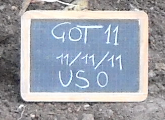
\includegraphics[width=0.6\textwidth]{catacom_1020_cutout.png}
\end{SCfigure}
Die im Beispielbild gezeigte Tafel stellt gewissermaßen ein Idealbild dar: Die Tafel nimmt einen relativ großen Teil des Originalbildes -- bei der Darstellung hier handelt es sich um einen Ausschnitt -- ein. Sie ist frontal vor der Kamera positioniert. Die Beleuchtung ist gut und indirekt. Keines der weiteren Bildelemente verdeckt die Tafel.
Diese Beschreibung impliziert schon die Problemfelder, die bei der Detektion beachtet werden müssen:
\begin{enumerate}
\item Die Tafel ist unter Umständen stark rotiert.
\item Die Distanz der Tafel zur Kamera und damit ihre Größe im Bild kann stark variieren.
\item Der Rahmen der Tafel kann teilweise verdeckt oder anderweitig durch Gegenstände überlagert sein.
\item Die Farbe des Tafelrahmens kann dazu führen, dass sie sich nicht klar vom Hintergrund abhebt, was die Detektion des äußeren Randes erschweren kann.
\item Unregelmäßigkeiten im Rahmen, die auf grobe Verarbeitung oder Abnutzung zurückzuführen sind, können die Detektion erschweren.
\item Die Beleuchtung kann zu Problemen führen. Grundsätzlich sind alle Fotos hell und gut ausgeleuchtet, direktes Licht kann sich aber negativ auf die Kontraste auswirken.
\item Weitere Gegenstände, die den Spezifika der Tafeln entsprechen, können im Bild vorhanden sein.
\end{enumerate}
Teilweise werden die hier genannten Probleme auch bei der Texterkennung wieder relevant. Auf diese und auf weitere wird an geeigneter Stelle zurückgegriffen.

\subsubsection{Tafelvergleiche}

Im Rahmen der Arbeit wurden weitere Tafeln exemplarisch dem Algorithmus unterzogen. Dabei handelte es sich um Aufnahmen der späteren Grabungen des Deutschen Archäologischen Institutes am Kapitol in Rom sowie um vergleichbare Fotos von Bodenuntersuchungen der Gruppe Terrestrische Ökohydrologie der Friedrich-Schiller-Universität Jena. Der ursprüngliche Gedanke dahinter war eine möglichst universale Detektion von Tafeln aller Art anzustreben. Während dieses Vorhaben aus Zeit- und Komplexitätsgründen ohnehin zum Scheitern verurteilt war, warf das weitere Material die Frage auf, wo die Grenze des technisch möglichen liegt, vor allem mit der hier letztlich gewählten Methodik.\\
Die Tafeln beider Projekte sollen im Folgenden kurz vorgestellt werden, um das Spektrum der Komplexität 
evtl. Vergleiche zu Tafeln aus späterer Grabung als Positivbeispiel:\\
besser gearbeitete Tafeln\\
besser lesbare Schrift\\
evtl. Vergleiche zu Tafeln der Bodenkunde als Negativbeispiel:\\
Tafel schwierig durch Form und Farbe\\
Klarsichthülle: Reflektion und Formveränderung\\
oft verdeckt\\

\subsection{Detektierungsmöglichkeiten}

\subsubsection{CNN}

CNN\\

Convolutional Neural Networks (CNN) Kurzdefinition\\

Coco und Coco bzw. Yolo Weights erklären\\

Code Herkunft erklären (Rücksprache Sellent bzgl. Quelle und Zitation etc.)\\

\subsubsection{Ergebnisse CNN}

Der Ansatz bei der Arbeit mit CNNs bestand in der Überlegung, dass die Tafeln bestimmten Objekten, wie beispielsweise Bücher oder Müslipackungen, ausreichend ähneln, um als solche erkannt zu werden. Prinzipiell wäre es auch möglich, ein eigenes Modell zu trainieren, dass auf die Erkennung der Tafeln zugeschnitten ist. Dieser Ansatz wurde hier nicht weiter verfolgt, da einerseits die vorliegende Datenmenge von knapp 1500 Bildern gering für ein solches Vorhaben ist und andererseits der Aufwand sehr groß wäre für ein Problem, das sich mit klassischen Methoden der Computer Vision ohne Weiteres lösen lässt.\\
Entsprechend wurden sowohl der YOLO, als auch der COCO object detector auf den Datensatz angewandt. Die Ergebnisse sind dabei wenig überzeugend.

\begin{SCfigure}[1][h!]
\caption{Eine beispielhafte Auswertung mit COCO-Weights: Es werden zwar durchaus Objekte erkannt, die Tafel ist aber nicht darunter. Die Objekte werden nicht korrekt erkannt, was aber bei dieser untypischen Fotografie nicht weiter verwunderlich ist.}
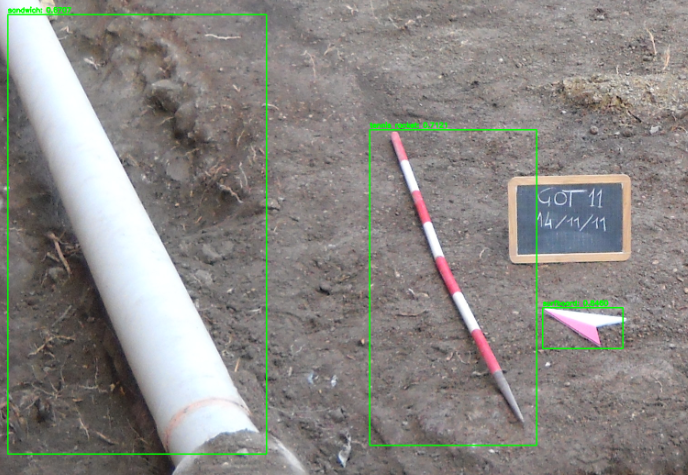
\includegraphics[width=0.5\textwidth]{coco_fail.PNG}
\end{SCfigure}

\begin{SCfigure}[1][h!]
\caption{Auffällig häufig ist die Klassifizierung des Nordungspfeils als Surfbrett. Diese ist aber nicht häufig und zuverlässig genug, um COCO zur Erkennung des Pfeils einzusetzen.}
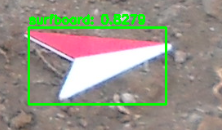
\includegraphics[width=0.5\textwidth]{coco_surfboard.PNG}
\end{SCfigure}

\begin{SCfigure}[1][h!]
\caption{Ähnlich wie bei COCO klassifiziert auch YOLO die Tafeln nur auf wenigen Bilder. Dann allerdings als Scheren...}
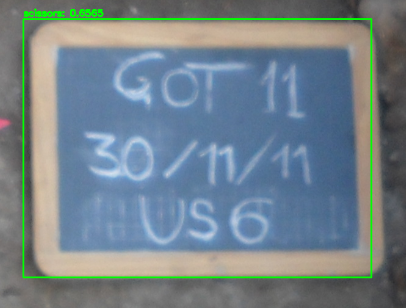
\includegraphics[width=0.5\textwidth]{scissors.PNG}
\end{SCfigure}

\begin{SCfigure}[1][h!]
\caption{... oder als Sportgerät. Die erhoffte Ähnlichkeit mit beschrifteten, rechteckigen Objekten wie Büchern besteht somit also nicht.}
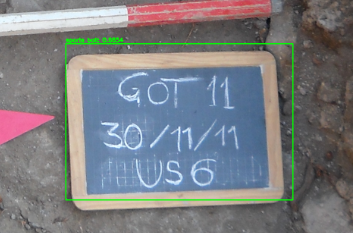
\includegraphics[width=0.5\textwidth]{sportsball.PNG}
\end{SCfigure}

\subsubsection{Ergebnisse Feature Detection}

theoretische Grundlagen Feature Detection\\

\subsubsection{Ergebnisse Feature Detection}

alten Code raussuchen, aufbereiten und präsentieren\\

\subsubsection{Contours}

Die \verb|Contours|-Funktion von OpenCV basiert darauf, dass alle benachbarten Punkte mit gleicher Farbe oder Intensität als Teil einer Kontur betrachtet werden (Quelle OpenCV doc). Der Algorithmus liefert also eine Liste von Punkten, die Grundlage einer Vektorgrafik sind. Der Parameter \verb|cv2.CHAIN_APPROX_SIMPLE| vereinfacht die Kontur, indem redundante Punkte entfernt werden. Als Input für Contours werden binarisierte Bilder empfohlen. Das sind Bilder, die in eine Grauskala umgewandelt  und anhand eines Thresholds, eines Grenzwertes, in ein reines Schwarz-Weiß-Bild transformiert wurden. Zur Binarisierung wurden im Verlauf der Entwicklung zwei Verfahren geschrieben, von denen eines de facto nicht mehr in Verwendung ist, der Vollständigkeit halber hier aber aufgeführt werden soll.
Das Kernproblem, das zu der parallelen Entstehung zweier Konzepte führte, waren vor allem falsch-positive Detektionen von Tafeln, also Fälle, in denen korrekterweise Rechtecke erkannt wurden, die aber keine Tafeln waren.
\begin{SCfigure}[1][h!]
\caption{Falsch-Positive: Hier werden korrekterweise Rechtecke detektiert, die allerdings keine Tafeln und somit uninteressant für die weitere Verarbeitung sind.}
\includegraphics[width=0.5\textwidth]{catacom_1023_adaptive.png}
\end{SCfigure}

\subsubsection*{Adaptiver Ansatz}
Der adaptive Ansatz heißt so aufgrund der Verwendung eines adaptiven Thresholds, der auf Bildausschnitten vorher festgelegter Größe gewissermaßen lokale Thresholds festlegt und so gut geeignet ist, um Bilder mit großen Unterschieden in der Helligkeit zu binarisieren, ohne dass wichtige Informationen verloren gehen (Quelle OpenCV doc). Da es bei dem vorliegenden Material, vor allem aufgrund von Schatten und direktem Sonnenlicht, große Helligkeitsunterschiede sowohl zwischen den Bildern als auch innerhalb eines einzelnen Bildes gibt, ist die Arbeit mit einem fixen Threshold schwierig und dieser Ansatz bot sich an. Allerdings entstand dadurch eine relativ große Zahl an falsch-positiven, wie oben zu sehen. So kam es zur Entwicklung des zweitens Ansatzes.\\
Die Umsetzung des adaptiven Ansatzes sieht wie folgt aus:
Als Input für die entsprechende Funktion werden das zu bearbeitende Bild und der dazugehörige Dateiname übergeben, der für die Nachverfolgung und den Output wichtig ist. Das Bild wird in eine Grauskala umgewandelt und in mit der Funktion \verb|scaleImage| auf eine Größe von 1000 Pixeln skaliert. Dieser Schritt erfolgt, um die Detektion durch kleinere Datenmengen zu beschleunigen und um durch die dadurch einheitliche Größe der Bilder präzisere Kriterien für die Rechtecksdetektion formulieren zu können. Das skalierte Bild wird jetzt mittels adaptiven Threshold binarisiert. Es folgt die eigentliche Rechtecksdetektion durch den Aufruf der Funktion \verb|rect_detect|, auf die später genauer eingegangen wird. Die so gewonnenen Konturen und entdeckten Rechtecke werden auf das skalierte Bild übertragen und der \verb|output|-Funktion übergeben. Die Rechtecke selbst, im Code als \verb|rois| (region of interest) bezeichnet, werden auf die ursprüngliche Bildgröße zurückskaliert und in das Hauptprogramm übergeben, damit die Bilder in ihrer höheren Ursprungsauflösung weiter bearbeitet werden können.
\begin{SCfigure}[1][h!]
\caption{Detektion mittels adaptiven Ansatz: Aus allen gefunden Konturen (rot) werden die Rechtecke ausgewählt (grün).}
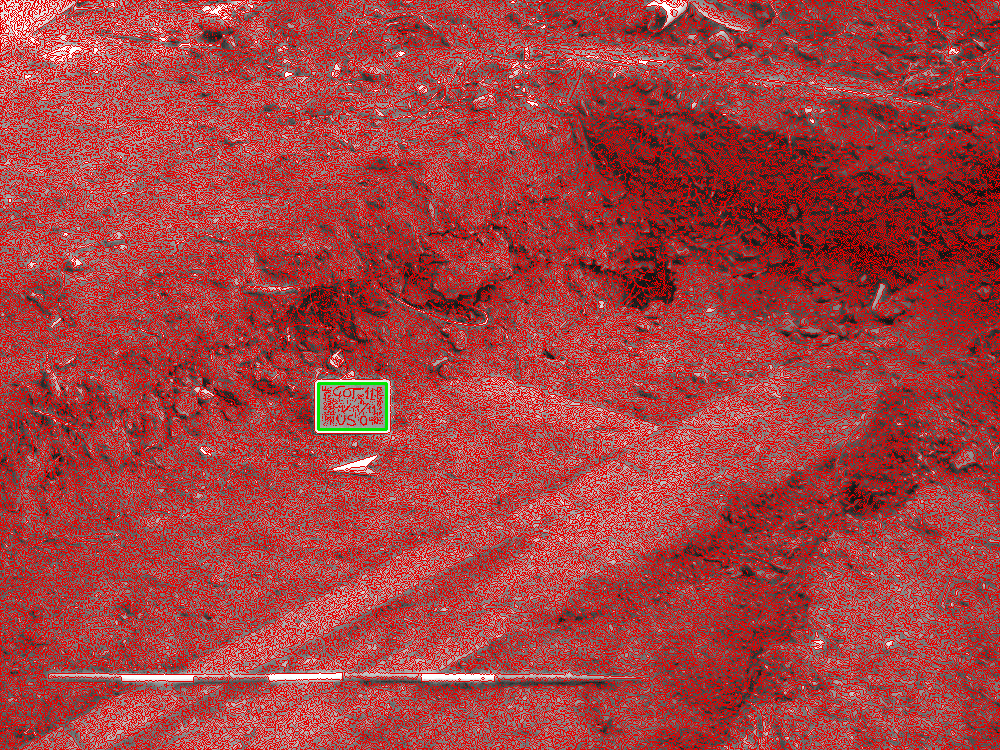
\includegraphics[width=0.5\textwidth]{catacom_1020_adaptive.png}
\end{SCfigure}

\subsubsection*{Iterativer Ansatz}
Der Iterative Ansatz ist danach benannt, dass durch ein Spektrum an Thresholds iteriert wird. In jedem dieser so entstandenen binären Bilder werden anschließend die Contours gesucht und aus diesen wiederum die Rechtecke ausgewählt. Die Idee dahinter war, dass die Falsch-Positiven oft weniger konstant in den Bildern detektiert wurden als die tatsächlichen Tafeln. Würde man also ein Bild mit verschiedenen Thresholds binarisieren sollte das Rechteck, dass in den meisten dieser binären Bilder entdeckt wird, die Tafel sein. In der Implementierung dieses Ansatzes werden von 20 bis 200 in Fünferschritten 37 Thresholds durchlaufen. Die Gleichheit zweier Rechtecke wird dabei mittels \textit{Intersection over Union} berechnet, deren Ergebnis sich der 1 nähert, je gleicher die Rechtecke in Position und Größe sind. Im Detail sieht das wie folgt aus: Aus den globalen Flags wird ein Wert für den minimalen Threshold übernommen. Wie bereits in dem adaptiven Verfahren wird das Bild in eine Grauskala umgewandelt. Beginnend beim minimalen Threshold (default = 20) werden die Bilder binarisiert und mit \verb|rect_detect| auf Rechtecke untersucht. Diese werden in der Liste \verb|allRois| gespeichert und der Threshold um 5 erhöht, bis der Wert von 200 erreicht ist.
Im Anschluss werden die Rechtecke in eine Liste von Dictionaries überführt. Das hat den Hintergrund, dass sich hier leicht und übersichtlich ein Keyword einfügen lässt, mit dem die Zahl ähnlicher Rechtecke gemessen werden kann. In zwei Schleifen wird diese Liste durchlaufen und so je zwei Rechtecke mittels \verb|intersection_over_union| miteinander verglichen. Wird ein Wert von über 0.9, also eine hohe Übereinstimmung, erzielt, wird das Keyword \verb|same| um eins erhöht.
Schließlich wird das Rechteck mit dem höchsten \verb|same|-Wert als ein Tafelfund betrachtet. Das weitere Verfahren ist wie beim adaptiven Ansatz: Das gefundene Rechteck wird auf das Bild übertragen und ausgegeben und dann ins Hauptprogramm zurückgegeben. Im Gegensatz zum adaptiven Ansatz ist hier eine Rückgabe mehrerer Rechtecke nicht möglich; Es wird immer genau ein Rechteck übergeben.
Tatsächlich können mit diesem Verfahren die Zahl der Falsch-Positiven reduziert werden, ohne das Problem allerdings ganz zu lösen. Generell lässt sich sagen, dass je öfter ein Rechteck in einer der Iterationen erkannt wird, desto größer ist die Wahrscheinlichkeit, dass es sich tatsächlich um eine Tafel handelt. Ab einem Wert von 20 liegt die Quote bei 100\%. Es gibt aber auch korrekt erkannte Tafeln, die nur in 6 der Iterationen detektiert werden und umgekehrt Falsch-Positive, die in bis zu 14 Iterationen vorkommen. Zwar handelt es sich hier jeweils um Ausreißer, das Problem bleibt jedoch bestehen. Empirisch hat sich gezeigt, dass alles unter 6 Iterationen mit Sicherheit keine Tafel ist und somit aussortiert werden kann. Wenige Ausreißer verhindern, dass diese Grenze nach oben gesetzt werden kann. Auch dieser Ansatz führte also nicht zum gewünschten Ergebnis.
\begin{SCfigure}[1][h!]
\caption{Falsch-Positive beim Iterativen Ansatz. Hier wurden in 14 Iterationen die Holzbretter als Rechteck identifiziert.}
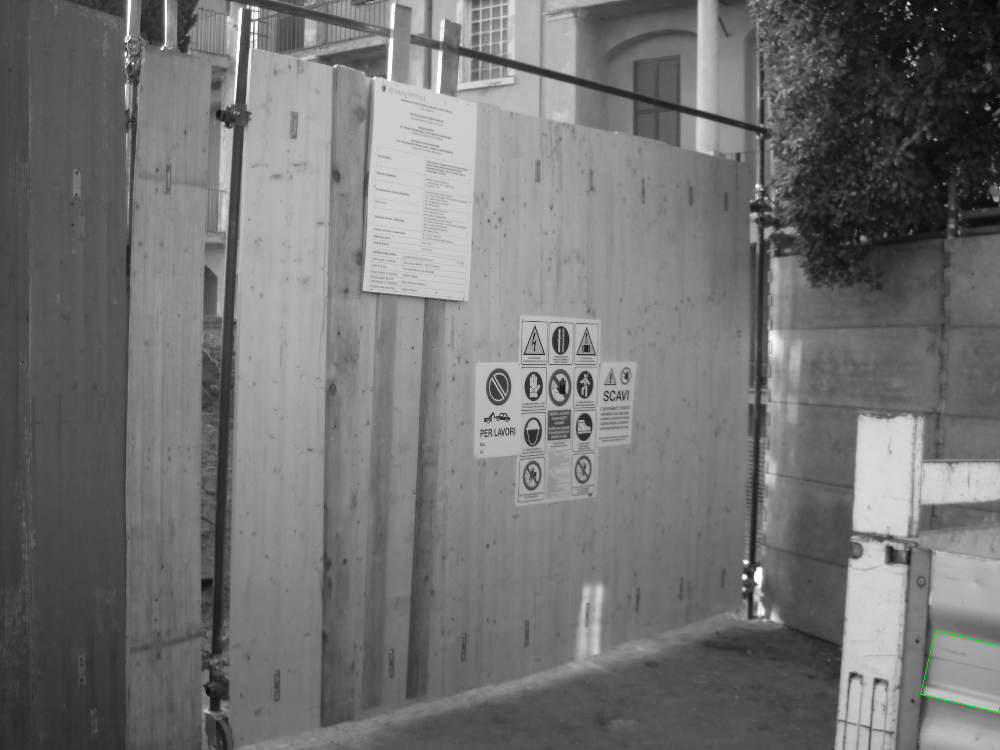
\includegraphics[width=0.5\textwidth]{catacom_1083_14.png}
\end{SCfigure}
\begin{SCfigure}[1][h!]
\caption{Direkte Sonneneinstrahlung macht die Erkennung schwierig, vor allem, da sich der Rahmen nicht mehr stark vom Schiefer abhebt. Nur in 6 Iterationen wurde diese Tafel erkannt.}
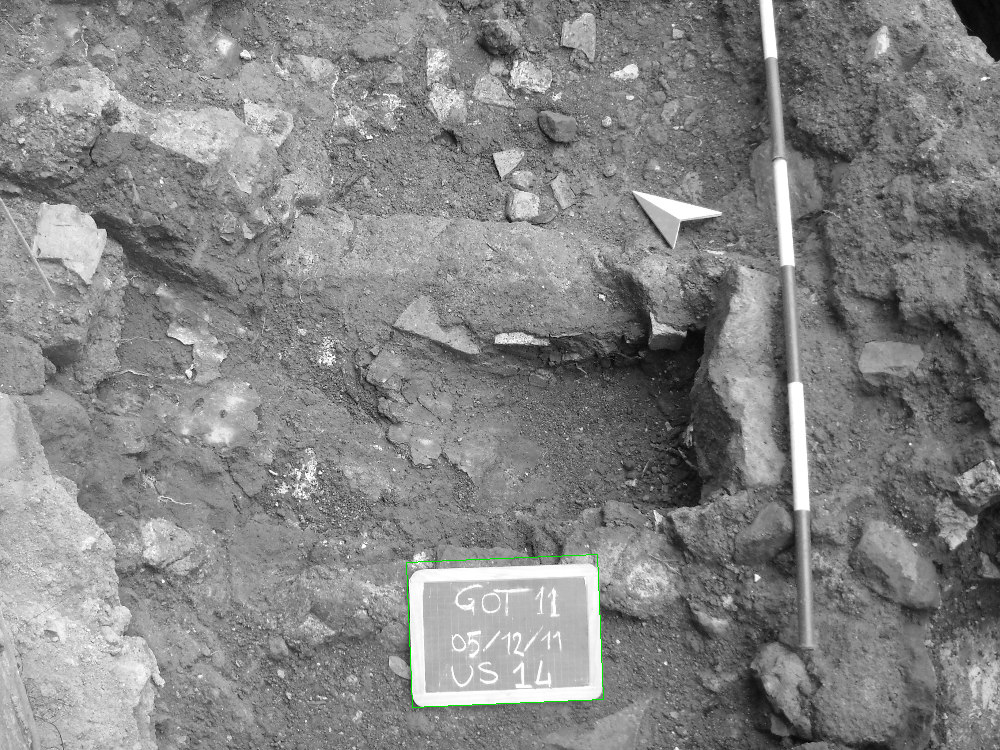
\includegraphics[width=0.5\textwidth]{catacom_1162_6.png}
\end{SCfigure}\\

\subsubsection{Rectangle Detection}

Die beiden vorgestellten Ansätze beziehen sich auf das Verfahren der Binarisierung. Die eigentliche Rechtecksdetektion wird von beiden aber in die Funktion \verb|rect_detect| ausgelagert. Das zugrundeliegende Verfahren ist dabei einfach gehalten: Mittels \verb|cv2.minAreaRect| wird das kleinstmögliche Rechteck um eine Kontur gelegt. Der Flächeninhalt dieses Rechtecks wird mit dem der Kontur verglichen. Gleichen sich die Flächen zu einem gewissen Grad -- bewährt hat sich hier eine Konturfläche von 85\% der Rechtecksfläche -- kann angenommen werden, dass es sich bei der Kontur um ein Rechteck handelt. Das Speicherformat dieser Rechtecke besteht in der Formel \verb|(x,y),(w,h), angle|. Das bedeutet, dass der Mittelpunkt der Rechtecke, ihre Breite und Höhe sowie der Rotationswinkel im Uhrzeigersinn gespeichert werden. 
Der ursprüngliche Gedanke war, weitere Auswahlkriterien möglichst bereits in der Binarisierung zu treffen. Da hier aber zunächst garantiert werden muss, dass kein mögliches Rechteck ausgeschlossen wird, also Falsch-Positive in kauf genommen werden müssen, um Falsch-Negative auszuschließen, entstehen hier widersprüchliche Anforderungen. Diese Priorisierung folgt daraus, dass eine erneute Prüfung einmal aussortierter Areale nicht möglich ist und diese für weitere Prozesse verloren sind.
Dieser Gedanke wurde jedoch verworfen. Stattdessen wurden die Auswahlkriterien, ab wann eine Kontur als gültiges Rechteck betrachtet, immer weiter verfeinert. Der folgende Code zeigt die zahlreichen Bedingungen, die zum Ausschluss einer Kontur als mögliche Tafel führen.
Zunächst werden alle Konturen mittels \verb|cv2.findContours| ermittelt. Aus diesen werden dann alle zu kleinen Elemente aussortiert: Was in der Fläche eine gewisse Größe unterschreitet kann keine Tafel sein, da diese immer eine gewisse Prominenz im Bild haben. Der nächste Schritt ist dann der bereits beschriebene Vergleich zwischen Fläche der Kontur und Fläche des kleinsten, die Kontur umfassenden Rechtecks. Als nächstes werden dann Rechtecke aussortiert, die einen großen Teil des Bildes -- über 90\% einer Kantenlänge -- einnehmen. Eine Tafel wird niemals diese Größe im Bild erreichen, stattdessen können hier Bilder aussortiert werden, die in ihrer Gesamtheit von einer Kontur eingerahmt sind und so zu Fehlern führten. Schließlich wird geprüft, ob die Seitenverhältnisse stimmen. Das geschieht anhand eines optionalen Templates. Dieses Template besteht aus einem Bild, das der Nutzer im Input-Ordner hinterlegen kann. Dieses Bild sollte optimale Bedingungen für eine Erkennung bieten, also eine gut sichtbare Tafel und keine Störobjekte und mögliche Falsch-Positive enthalten. Die Tafel auf diesem Bild wird gleich zu Beginn des Programmes erkannt und daraus das Seitenverhältnis der Tafel berechnet. Dieses Seitenverhältnis kann mit dem jedes Rechtecks verglichen werden. Weichen die Werte zu stark voneinander ab, kann es sich nicht um eine der gesuchten Tafeln handeln. Eine gewissen Abweichung muss aber durch die Rotation der Tafeln in Kauf genommen werden. Dieser Prozess könnte verbessert werden, indem man ihn in spätere Bereiche des Programmes verschiebt, an denen die Rotation herausgerechnet wird. Da der Vorgang allerdings schon ausreichend gut funktioniert ist der zusätzliche Aufwand nicht notwendig.

\subsubsection{Ergebnisse Rectangle Detection}

\subsubsection{Crop-Verfahren}

Nach der Detektion der Tafeln besteht der nächste Schritt darin, sie aus dem Restbild herauszulösen, um sie an die Texterkennung weiterleiten zu können. Auch hier gibt es wieder einige Faktoren zu beachten:
\begin{enumerate}
\item Die gefundenen Rechtecke geben nur ungefähr Größe und Form der Tafeln wieder.
\item Die eigentliche Form des Rahmens ist eher unregelmäßig statt perfekt rechteckig. Das ist durch die abgerundeten Ecken sowie Abnutzungen des Rahmens bedingt.
\item Die Tafeln können entlang der drei Achsen rotiert sein. Durch die zweidimensionale Abbildung auf der Fotografie können die Formen letztlich eher einem Parallelogramm als einem Rechteck entsprechen. Diese Verzerrung sollte ausgeglichen werden.
\end{enumerate}


\subsubsection*{Simple Crop}

Wie bereits zuvor wurde auch diese Problematik über mehrere Wege angegangen. Der erste und einfachste Weg, im Programm als \verb|simple_crop| bezeichnet, besteht in einer einfachen Transformation des gefundenen Rechtecks in eigenständiges Bild. Das Ergebnis ist also eine Rotation und Vergrößerung der Tafel. Erreicht wird das mittels \verb|cv2.getPerspectiveTransform|, einer Bibliotheksfunktion, die ein Set von Punkten auf neue Koordinaten projiziert und die Bereiche zwischen den Punkten entsprechen transformiert. Für diesen Ansatz werden aus bekannten Kennzahlen der Rechtecke (Koordinaten des Mittelpunkts, Breite, Höhe, Rotationswinkel) via die Eckpunkte berechnet. Als Zielkoordinaten wird ein Rechteck gewählt, das in Höhe und Breite dem gefundenen Rechteck entspricht. Das Ergebnis der Transformation ist letztlich vor allem die Rotation des Bildes.
Das so erhaltene Bild wird um 90° gedreht, wenn die Höhe größer ist als die Breite des Bildes. So soll erreicht werden, dass die Tafeln alle richtig herum, d.h. mit der korrekten Leserichtung des Textes, ausgegeben werden.
Schließlich werden die Images auf eine einheitliche Größe (1000px Breite) skaliert. Ursprünglich war hier vorgesehen, das aspect ratio mit einzubeziehen, um die Höhe passend zur Breite zu bemessen. Dieser Ansatz verschlechtert jedoch die spätere Texterkennung, da die Buchstaben gestaucht werden, wenn der Rechtecksausschnitt die Tafel nicht perfekt erkannt hat und daher über ein anderes Seitenverhältnis verfügt als die Idealvorlage. Daher wird das Seitenverhältnis des Ausschnitts beibehalten und die Höhe entsprechend berechnet.
Eine Modifikation dieser Herangehensweise, bei der die gefundene Kontur innerhalb des Rechtecks in eine Maske umgewandelt wird, die wiederum als Basis für den Bildausschnitt dient und somit alle Elemente, die die Kontur umgeben, ausblendet, wurde verworfen. Das geschah aufgrund der schlechteren Ergebnisse bei der späteren Texterkennung.

\begin{SCfigure}[1][h!]
\caption{Nahezu perfekte Erkennung des Rechtecks und somit auch ein gutes Ergebnis bei simple crop. Es ist weder Rand noch Hintergrund zu sehen, die Form entspricht der eines Rechtecks.}
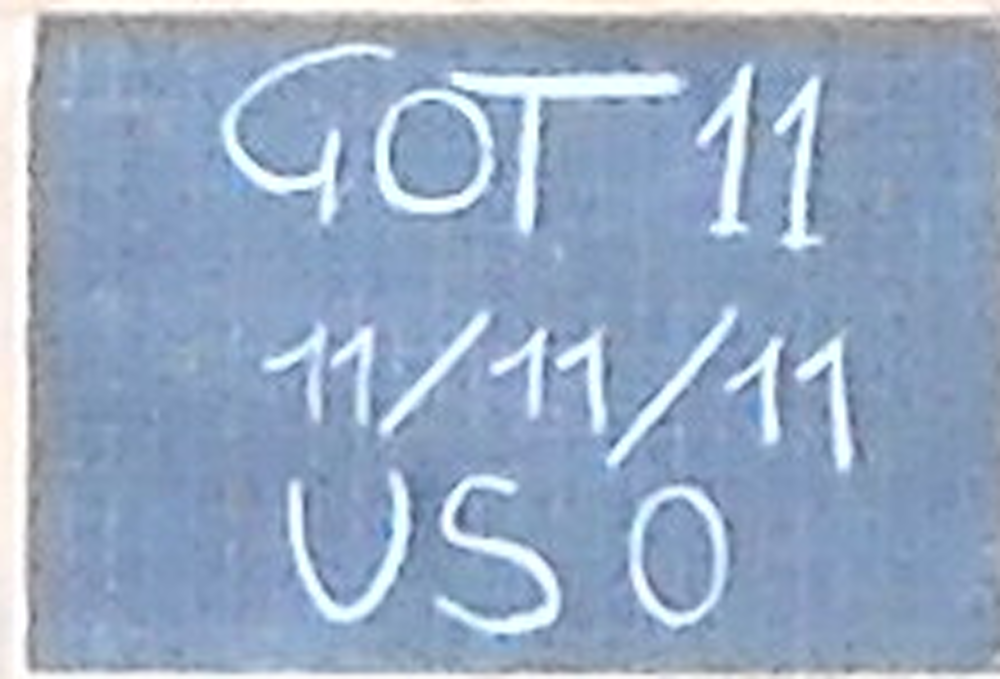
\includegraphics[width=0.5\textwidth]{good_crop.png}
\end{SCfigure}

\begin{SCfigure}[1][h!]
\caption{In diesem Beispiel hat cv2.contours den äußeren Rand des Rahmens als Kontur identifiziert. Bedingt durch die Rotation der Tafel bildet sie, zweidimensional abgebildet, eher ein Parallelogramm. Das kleinstmögliche Rechteck, das die Form umgibt, schließt somit auch Teile des Hintergrunds mit ein.}
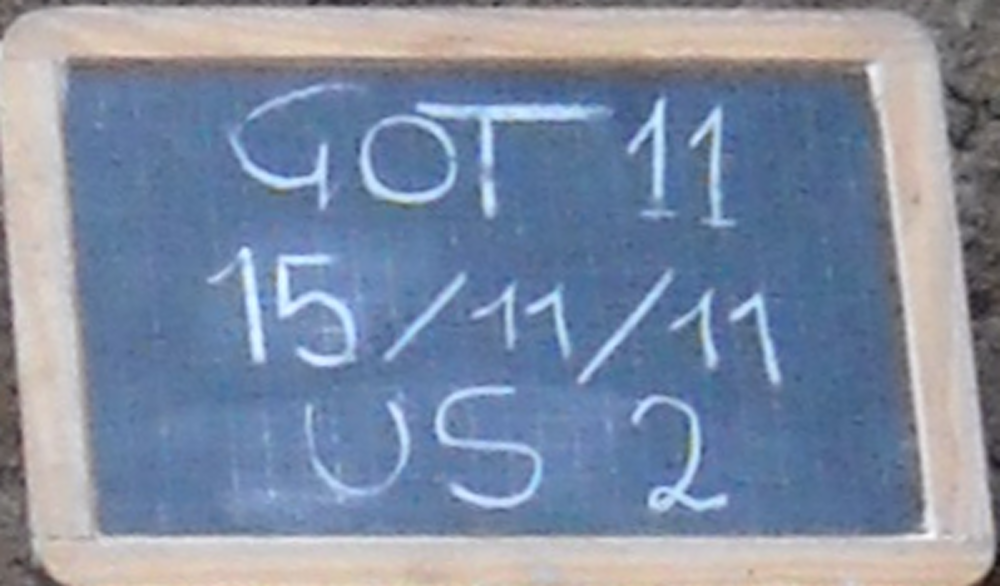
\includegraphics[width=0.5\textwidth]{bad_crop.png}
\end{SCfigure}

\subsubsection*{Hough Crop}

Das bisher vorgestellte \verb|simple crop|-Verfahren muss als relativ grob betrachtet werden. Verbesserung sollte sich einstellen, wenn statt der Eckpunkte der Rechtecke die Eckpunkte der Tafeln selbst erkannt werden könnten. Würden diese dann für die Transformation mittels \verb|cv2.getPerspectiveTransform| verwendet, könnte die Rotation der Tafeln ausgeglichen werden.
Zentral für diese Vorgehensweise ist die Hough\footnote{Gesprochen: [h\textturnv{}f]}-Transformation, ein Verfahren zur Erkennung geometrischer Figuren in binarisierten Bildern (Vgl. Hough 1962 \cite{houghpatent}). Mit diesem Verfahren -- bzw. mit der darauf basierenden Funktion \verb|cv2.HoughLines| -- könnten die einzelnen Seiten der Tafeln als Linien erkannt werden. Allerdings benötigt die Funktion einiges an pre-processing, auf das im Folgenden näher eingegangen werden soll.
Der erste und offensichtliche Schritt besteht darin, das Bild zu binarisieren. Dabei entstehen Probleme, wie sie bereits zuvor bei der Rechtecksdetektion festgestellt wurden: die Bilder, vor allem die Regionen mit den Tafeln darauf, sind zu unterschiedlich beleuchtet, um einen einheitlichen Threshold festlegen zu können, der die Kanten der Tafeln sauber vom Hintergrund trennen kann. Direkte Korrelationen zwischen den Farbwerten -- sei es im RGB-Bereich oder auf der Grauskala -- und dem optimalen Threshold konnten nicht festgestellt werden. Daher wurde hier der gleiche Weg gewählt wie bereits zuvor beim iterativen Ansatz in der Tafelerkennung: Beginnend bei einem Wert von 150 (der per globaler Flag jederzeit angepasst werden kann) wird der Threshold um Fünf verringert, bis er den Wert von 100 erreicht. Wurde in keinem der Durchläufe das Hough-Verfahren erfolgreich abgeschlossen, wird stattdessen \verb|simple_crop| angewendet.
Die Binarisierung selbst erfolgt dabei aber nicht auf dem ganzen Bild, sondern auf einem Bildausschnitt. Ursprünglich entsprach dieser dem um 30\% vergrößerten Rechteck aus \verb|rect_detect|. Damit sollte erreicht werden, dass auch in den Rechtecken, die bereits in erster Instanz große Übereinstimmungen mit den Tafeln hatten, die Kanten mittels Hough-Algorithmus erkannt werden können. Auch die Problematik der durch Rotation nicht rechteckig abgebildeten Tafeln, die immerhin Anlass für diesen komplexeren Ansatz waren, konnte so besser behandelt werden, da diese, bedingt durch ihre Form, nicht immer ganz in den Rechtecksausschnitten in ihrer ursprünglichen Größe enthalten waren. Gleichzeitig war diese Beschneidung nötig, um zu verhindern, dass Objekte mit geraden Kanten im Hintergrund -- wie Türen, Fenster, Messstäbe -- in der Linienerkennung eine Rolle spielen und somit das Problem der Falsch-Positiven wieder auftritt. In Einzelfällen bleibt dieses Problem bestehen, wenn einer der genannten Gegenstände nahe der Tafel platziert wurde.

\begin{SCfigure}[1][h!]
\caption{Die Nähe des Messstabes kann dazu führen, dass dieser als Linie erkannt wird und das Bild somit verzerrt.}
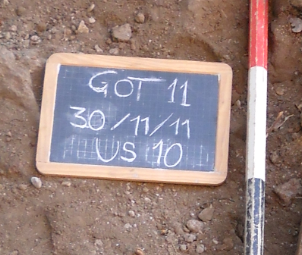
\includegraphics[width=0.5\textwidth]{messstab.PNG}
\end{SCfigure}

Dieses Problem kann vollkommen umgangen werden, wenn als Grundlage für die Linienerkennung nicht das volle Bild genutzt, sondern nur der Bereich der ursprünglich detektierten Kontur berücksichtigt wird. Diese Vorgehensweise, die bereits bei \verb|simple_crop| erprobt, dort allerdings verworfen wurde, verhindert hier vollständig die Linienerkennung bei nicht zur Tafel gehörigen Kanten.
Auch wenn die grundsätzliche Binarisierung damit abgehandelt ist, müssen weitere Schritte in diesem Kontext unternommen werden. Durch die unregelmäßige Struktur des Tafelrahmens sowie Artefakte, die durch die bisherige Bearbeitung (rotieren, skalieren, beschneiden) entstanden sind, kann es passieren, dass die Rahmen auf den Bildern nicht ausreichend gerade sind, um als Linien erkannt zu werden. Ausgeglichen wird das durch mehrere Filterverfahren -- \verb|cv2.bilateralFilter|, \verb|cv2.fastNlMeansDenoising| und \verb|cv2.GaussianBlur|. Ursprünglich musste an dieser Stelle das \textit{skeleton} des Bildes gezogen werden. Dafür werden mittels \verb|cv2.erode| die Objekte auf dem Bild immer weiter in reduziert, bis sie nur noch die Breite eines Pixels haben. Dieses Verfahren konnte die Unregelmäßigkeiten im Rahmen endgültig ausgleichen. Der Nachteil bestand darin, dass die Linen, die durch die Hough-Transformation erkannt wurden, immer in der Mitte das Rahmens lagen, da sich hier natürlich das \textit{skeleton} befindet. Das so ausgeschnittene Bild enthielt somit große Teile des Rahmens, was sich negativ auf die Texterkennung auswirkt. Dieses Problem konnte ebenfalls durch den Umstieg auf die ausgeschnittenen Konturen gelöst werden: Das Erzeugen des \textit{skeleton} ist nicht mehr notwendig. Ob der Rahmen zu sehen ist, hängt jetzt von der gefundenen Kontur ab. Da oft sowohl der innere, als auch der äußere Rand des Rahmens als Kontur erkannt wird, stellt dieser nur noch selten ein Problem dar.
